\documentclass[]{report}   % list options between brackets        
\usepackage{graphicx}      % list packages between braces
\graphicspath{ {Images/} }

% type user-defined commands here

\begin{document}

\title{CAB420 Assignment 1}   % type title between braces
\author{Jarrod Williams (n9722068) and Madeline Miller (n9342401)}         % type author(s) between braces
\maketitle

\chapter{Theory}

Given the following equation,

$$L(w)=-\sum_{i=1}^{N}log(\frac{1}{1+e^{y_i(w^Tx_i+b)}})+\lambda||w||_2^2$$

\section{Finding the Partial Derivative}
Finding the partial derivative $$\frac{\partial L}{\partial w_j}$$

$$\frac{\partial L}{\partial w_j}(-\sum_{i=1}^{N}log(\frac{1}{1+e^{y_i(w^Tx_i+b)}})+\lambda||w||_2^2)$$

As the regulator at the end of the function is a squared L2 norm, it can be derived trivially.

$$\frac{\partial L}{\partial w_j}(-\sum_{i=1}^{N}log(\frac{1}{1+e^{y_i(w^Tx_i+b)}}))+2\lambda w_j$$

Simplify,

$$\frac{\partial L}{\partial w_j}(\sum_{i=1}^{N}log(1+e^{y_i(w^Tx_i+b)}))+2\lambda w_j$$

Using the chain rule,

$$\sum_{i=1}^{N}\frac{\frac{\partial L}{\partial w_j}(1+e^{y_i(w^Tx_i+b)})}{1+e^{y_i(w_jx_{i,j}+b)}}+2\lambda w_j$$

$$\sum_{i=1}^{N}\frac{\frac{\partial L}{\partial w_j}(1)+\frac{\partial L}{\partial w_j}(e^{y_i(w^Tx_i+b)})}{1+e^{y_i(w_jx_{i,j}+b)}}+2\lambda w_j$$

$$\sum_{i=1}^{N}\frac{\frac{\partial L}{\partial w_j}(e^{y_i(w^Tx_i+b)})}{1+e^{y_i(w_jx_{i,j}+b)}}+2\lambda w_j$$

Using the chain rule again,

$$\sum_{i=1}^{N}\frac{y_ix_ie^{y_i(w^Tx_i+b)}}{1+e^{y_i(w_jx_{i,j}+b)}}+2\lambda w_j$$

\section{Finding the Second Partial Derivative}
Finding the second partial derivative $$\frac{\partial^2 L}{\partial w_j\partial w_k}$$

$$\frac{\partial^2 L}{\partial w_j\partial w_k}=\frac{\partial}{\partial w_k}(\sum_{i=1}^{N}\frac{y_ix_ie^{y_i(w^Tx_i+b)}}{1+e^{y_i(w_jx_{i,j}+b)}}+2\lambda w_j)$$

$$\frac{\partial}{\partial w_k}(\sum_{i=1}^{N}\frac{y_ix_ie^{y_i(w^Tx_i+b)}}{1+e^{y_i(w_jx_{i,j}+b)}})$$

$$\sum_{i=1}^{N}\frac{y_ix_i(\frac{\partial}{\partial w_k}e^{y_i(w^Tx_i+b)})}{1+e^{y_i(w_jx_{i,j}+b)}}$$

Using the chain rule,

$$\sum_{i=1}^{N}\frac{e^{y_i(w_kx_i+b)}y_i^2x_i(\frac{\partial}{\partial w_k}(w^Tx_i+b))}{1+e^{y_i(w_jx_{i,j}+b)}}$$

$$\sum_{i=1}^{N}\frac{e^{y_i(w^Tx_i+b)}y_i^2x_iw_kx_i+b}{1+e^{y_i(w_jx_{i,j}+b)}}$$

$$\sum_{i=1}^{N}\frac{e^{y_i(w^Tx_i+b)}y_i^2x_i^2w_k+b}{1+e^{y_i(w_jx_{i,j}+b)}}$$

\section{Proving it's a convex function}

A function can be defined as convex if the Hessian matrix is positive semi-definite. This is defined as,

$$a^THa\equiv\sum_{j,k}a_ja_kH_{j,k}\geq0$$

Where,

$$H_{j,k}=\frac{\partial^2L}{\partial w_j\partial w_k}$$

Using proof by contradiction, 




\chapter{Practice}


\section{Features, Classes, and Linear Regression}
%%%%%%%%%%%%%%%%%%%%

\begin{center}
	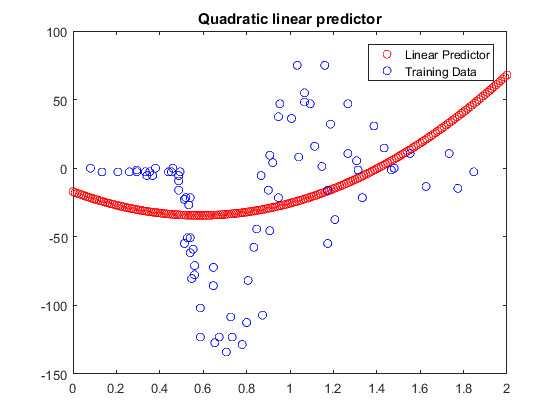
\includegraphics[width=35em]{2_1_Figure_1.png}
\end{center} 
{Figure 1: Quadratic linear predictor.} \\
{The Mean Squared Error for training data was $2178.55$.} \\
{The Mean Squared Error for test data was $1463.34$.} \\

\begin{center}
	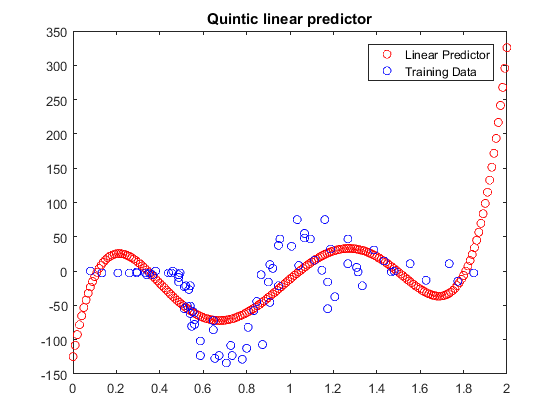
\includegraphics[width=35em]{2_1_Figure_2.png}
\end{center} 
{Figure 2: Quintic (Fifth-degree) linear predictor.} \\
{The Mean Squared Error for training data was $1254.61$.} \\
{The Mean Squared Error for test data was $754.17$.} \\


\section{kNN Regression}
\section{Hold-out and Cross-validation}
\section{Nearest Neighbor Classifiers}
%%%%%%%%%%%%%%%%%%%%

(a) Plot the data by their feature values, using the class value to select the color.
\begin{center}
	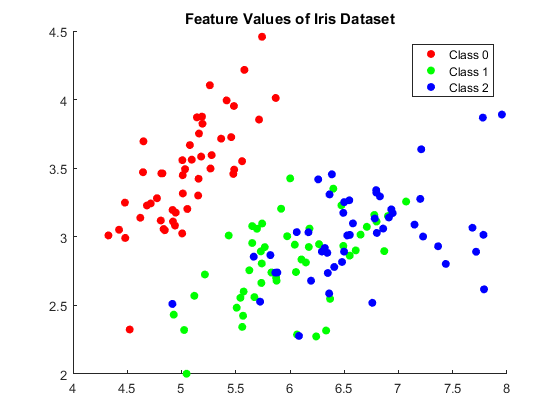
\includegraphics[width=35em]{2_4_Figure_1.png}
\end{center} 
(b) Use the provided $knnClassify$ class to learn a 1-nearest-neighbor predictor. Use the function $class2DPlot(learner,X,Y)$ to plot the decision regions and training data together.
\begin{center}
	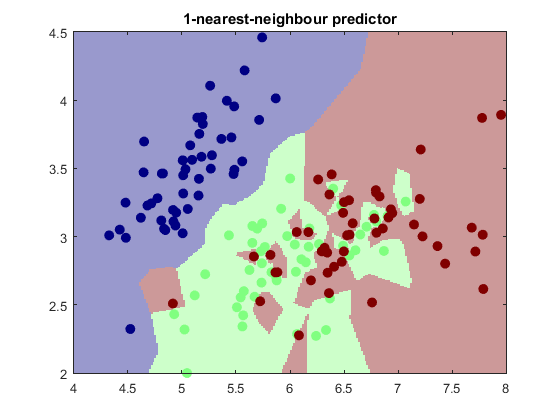
\includegraphics[width=35em]{2_4_Figure_2.png}
\end{center} 
(c) Do the same thing for several values of k (say, [1, 3, 10, 30]) and comment on their appearance.
\begin{center}
	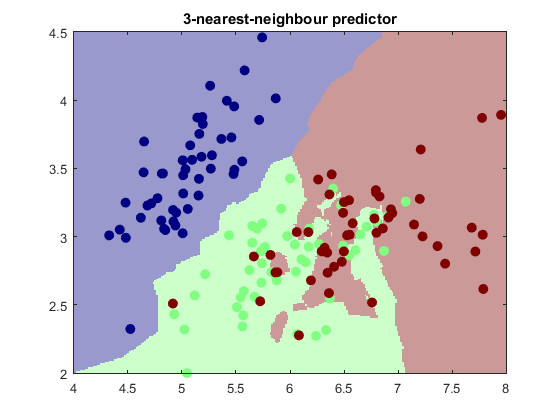
\includegraphics[width=35em]{2_4_Figure_3.png}
\end{center} 
\begin{center}
	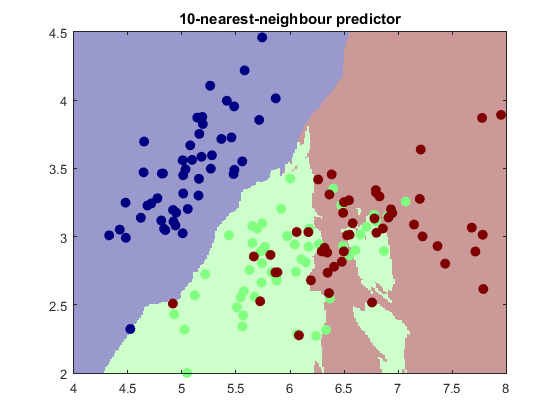
\includegraphics[width=35em]{2_4_Figure_4.png}
\end{center} 
\begin{center}
	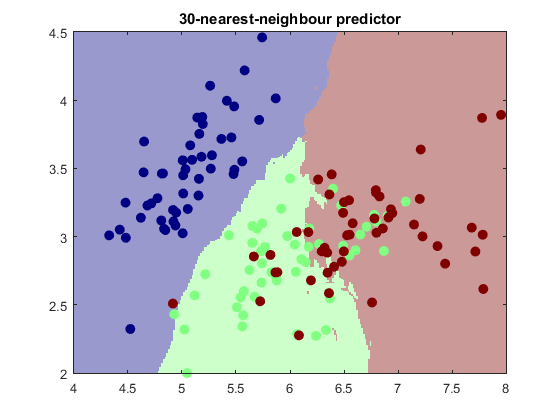
\includegraphics[width=35em]{2_4_Figure_5.png}
\end{center} 
{As the value of $k$ increases, so does the definition of the decision regions. At small values of $k$, under-fitting occurs. At large values of $k$, over-fitting occurs.}
\\~\\
{(d) Now split the data into an 80/20 training/validation split. For k = [1, 2, 5, 10, 50, 100, 200], learn a model on the 80$\%$ and calculate its performance ($\#$ of data classified incorrectly) on the validation data.}
\begin{center}
	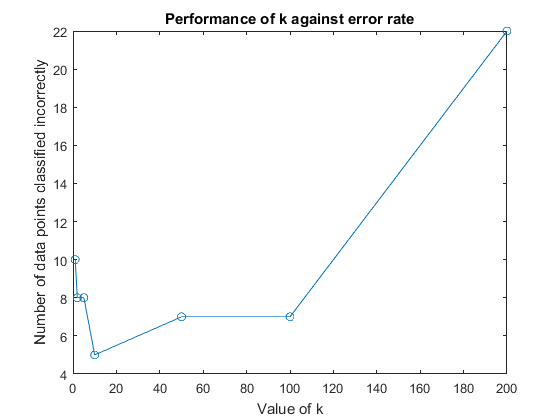
\includegraphics[width=35em]{2_4_Figure_6.png}
\end{center} 
{What value of k appears to generalize best given your training data? Comment on the performance at the two endpoints, in terms of over- or under-fitting.} \\~\\
{Where small values of $k$ underfit (1,3,5) and large values overfit (100,200), where $k = 10$ appears to generalise best.}



\section{Perceptrons and Logistic Regression}

\end{document}
